% !TeX root = ../main.tex
% Add the above to each chapter to make compiling the PDF easier in some editors.

\chapter{Implementation of vECU Setup}\label{chapter:Implementation}
In this chapter, we explore the practical implementation of the vECU setup as part of this thesis. The chapter provides a comprehensive and detailed account of each step involved in the process, ensuring a clear understanding of how the virtual ECU environment was constructed. It not only covers the technical aspects of the setup but also delves into the various challenges and complexities encountered along the way. Additionally, the chapter discusses the different strategies and solutions that were considered to overcome these obstacles, offering insights into the decision-making process. Finally, it outlines the rationale behind the final approach that was chosen, explaining why it was deemed the most effective solution for achieving the project’s goals.

\section{vCAN to SilKit Adapter}
After successfully building the application component of the vECU as a shared object in Linux using vVirtualTarget and establishing a connection between the SUTRunner and the SIL Kit registry, as discussed in the previous chapter, the next major challenge was to facilitate seamless communication between the vECU and external testing tools. This was particularly challenging because most of the testing software used at BMW, such as ECU-test \cite{ecu_test} and Esys, operates on Windows and relies on sending and receiving UDS requests and responses via a CAN bus to interact with the ECU. To bridge this communication gap, a specialized adapter called the "\textbf{vCAN\_To\_SILKit}" adapter was developed, which connects the virtual CAN bus to the SIL Kit registry, enabling smooth communication. ~\autoref{fig:test_setup} provides a visual representation of the entire test environment, highlighting the role of the adapter.

The "\textbf{vCAN\_To\_SILKit}" adapter is a crucial tool designed to  facilitate the interaction between the vECU and the testing software. The process to set up this adapter involves several key steps:


\begin{enumerate}
\item \textbf{Setting up the Virtual CAN Interface}: A virtual CAN interface is first configured on the Windows system using the Vector Hardware Configuration tool.
\item \textbf{Launching the "vCAN\_To\_SILKit" Adapter}: The adapter is then launched, binding to the virtual CAN interface on one side via the xlAPI interface, while on the other side, it connects to the SIL Kit as a participant in the simulation environment.
\item \textbf{Connecting SUTRunner to SIL Kit}: Once the adapter is operational, the SUTRunner software is started, and its connection to the SIL Kit registry is established, ensuring that all components are in sync.
\item \textbf{Running ECU-test}: With all connections successfully in place, the ECU-test software can be executed to transmit and receive CAN messages to and from the vECU through the "\textbf{vCAN\_To\_SILKit}" adapter, enabling comprehensive testing and validation of the vECU setup.
\end{enumerate}

This setup allows the ECU-test to interact with the virtual CAN interface, which is then bridged to the SIL Kit CAN bus, enabling testing and validation of the ECU without the need for physical hardware.

\subsection{Adapter to silkit}
The initial step in connecting the adapter to the SIL Kit registry involves creating a simulation participant. This is achieved using the "\textbf{SilKit::CreateParticipant}" function, where the participant is named "\textbf{vCAN\_To\_SILKit\_Adapter}", and both the "\textbf{registryUri}" and participant configuration are specified.

Once the "\textbf{IParticipant}" is established, a lifecycle service is created to manage the workflow and state transitions of this simulation participant. The lifecycle service is essential as it provides access to the time synchronization service, allows for the registration of callbacks for state changes, queries the participant’s current state, and issues commands to transition between states.

With the "\textbf{IParticipant}" instance in place, various SIL Kit services can be created and accessed. One of the critical services for this adapter is the CAN Service API, which offers a CAN bus abstraction via the "\textbf{ICanController}" interface. The CAN controller is instantiated by calling "\textbf{CreateCanController}", where the controller and network names are provided.

This "\textbf{ICanController}" is then passed as an argument to the "\textbf{create}" function, which is responsible for establishing the connection with the virtual CAN (vCAN) side. Once the setup is complete, the simulation can be initiated using the "\textbf{StartLifecycle}" method, which runs the simulation until it is either stopped or aborted. \cite{sil_kit_docs}


\subsection{CAN connection implementation}
This subsection provides a comprehensive overview of the process involved in implementing the connection to the virtual CAN (vCAN) network. 

At the heart of this connection lies the "ClassicalCanConnectionImpl" struct, which serves as the core component responsible for handling the intricate details of CAN message management. This struct is designed to effectively control the flow of CAN messages, ensuring they are accurately transmitted from the vCAN network to the SIL Kit network and vice versa. 

In ~\autoref{lst:can_connection}, the definition of the ClassicalCanConnectionImpl struct is presented. The listing not only outlines the structure of the implementation but also provides insights into how each function within the struct contributes to the overall process of CAN message management. 

\newpage

\begin{lstlisting}[caption={The ClassicalCanConnectionImpl struct.}, label={lst:can_connection}]
struct ClassicalCanConnectionImpl
{
public:
    ClassicalCanConnectionImpl() = default;
    ~ClassicalCanConnectionImpl() = default;

    //converts the CAN message from XLevent to a silkit CAN frame 
    CanFrame XLTOSILKIT(XLevent* event);

    // Writes the SIL Kit CanFrame to the vCAN
    void WriteToXL(XLportHandle portHandle, XLaccess accessMask, const CanFrame& SilkitFrame);

    // Handles received frames from the vCAN and sends them on the SIL Kit 
    void HandleReceivedCanFrameFromVirtualCanDevice(ICanController* canController,SilKit::Services::Logging::ILogger* logger, XLevent* event);

private:
    // Temporarily stores the CAN frame that is to be sent to the vCAN device
    XLevent _frameToVCAN;
};
\end{lstlisting}

\subsection{Adapter to vCAN}
  
This subsection delves into the other crucial aspect of the adapter: the connection to the virtual CAN (vCAN) network via the XL API. The integration between the SIL Kit API and the XL API begins with the create function, where the foundational connection is established. Within this function, an instance of the "\textbf{ClassicalCanConnectionImpl}" struct is created to manage the communication process.

The first step in this process is to initialize a virtual CAN connection. This involves several critical actions: opening an XL driver, retrieving the application configuration, opening the necessary port, and finally, activating the channel. These steps ensure that the vCAN is ready to transmit and receive CAN messages. \cite{xl_driver_library_manual}

On the transmission side, sending CAN messages from the SIL Kit to the vCAN is handled by the WriteToXL function within the "\textbf{ClassicalCanConnectionImpl}" struct. This function is linked to the SIL Kit by passing it to the AddFrameHandler function within the "\textbf{ICanController}", facilitating smooth communication between the two APIs.

For receiving messages, the process is managed by the ReceiveThread function, which operates in a continuous loop on a separate thread. This thread listens for incoming CAN messages using the xlReceive function. Upon receiving a message, it invokes the "\textbf{HandleReceivedCanFrameFromVirtualCanDevice}" function within the "\textbf{ICanController}", ensuring that messages are efficiently transferred from the vCAN to the SIL Kit network.

\subsection{Optimizations within the adapter}
To enhance the efficiency of CAN message transmission through the adapter, several key optimizations were implemented. These optimizations focused on reducing overhead and improving the speed of data transfer.

One significant optimization involved disabling receipt acknowledgments when a message is transmitted or when it is queued for transmission. By eliminating these acknowledgments, the system reduces unnecessary overhead, thereby accelerating the message transfer process.

Another critical optimization was applied to the receive thread. Originally, this thread continuously ran in an infinite loop, constantly checking for incoming messages. To eliminate the inefficiency of busy waiting, the thread was modified to wait for notifications from the receive queue. This was achieved using the "\textbf{xlSetNotification}" function, which configures the queue level for notifications on the specified port and returns a notification handle. This handle, linked to an auto-resetting Windows event, remains valid until the port is closed. By relying on event-driven notifications rather than constant polling, this approach significantly reduces CPU usage and enhances the overall performance of the adapter.

\section{A Unified Virtual Simulation}
In \autoref{section:ECU_architecture}, we discussed the three distinct software components of the ECU: the Application, the Boot Manager (BM), and the Bootloader (BL). A significant challenge in this project was the inability to virtualize these components as a single entity due to the limitations of our available software, which only allows for the virtualization of each software part separately. As a result, each component operates as an independent shared object within its own isolated simulation.

This separation presented a major obstacle, as it prevented the seamless integration and interaction of these components, which is essential for realistic testing and validation. In a physical ECU, the Boot Manager typically initializes some shared data, and controls the flow between the Application and the Bootloader, making it crucial for the virtual environment to replicate this behavior \cite{embeddedartistry_before_main}. Therefore, a unified simulation environment needed to be developed, one that could integrate all three software parts into a single cohesive simulation. This environment would not only have to manage the shared resources among the different components but also enable the Boot Manager to dynamically control which main function—whether the Application or the Bootloader—should be executed.

This section provides a detailed account of these approaches, discussing the various options that were considered, the reasoning behind each, and the iterative process that led to the final solution. \autoref{fig:vECU_setup} shows the desired vECU setup that can simulate the behavior of the actual ECU. 

\begin{figure}[htpb]
  \centering
  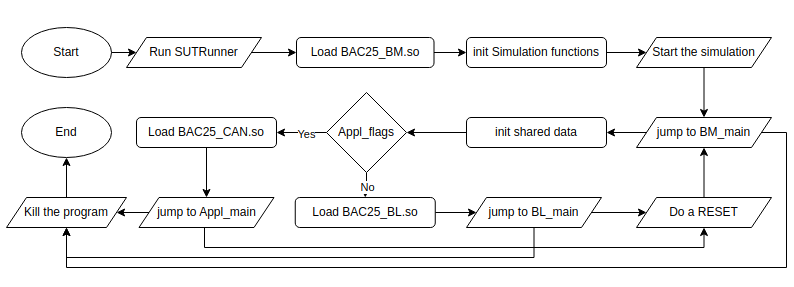
\includegraphics[width=1\textwidth]{figures/complete_setup.PNG}
  \caption{Interaction between the Application, BL, and Bm indise the vECU.} \label{fig:vECU_setup}
\end{figure}

\subsection{Initial Concept: Sequential Simulation Switching}
When initially considering how to manage the transition between the different software components of the ECU—the Application, Boot Manager (BM), and Bootloader (BL)—one approach that seemed straightforward was to handle these transitions by sequentially stopping and starting separate simulations. For example, once the Boot Manager completed its task, the idea was to halt its simulation and then initiate the simulation for the Application, and so forth.

At first glance, this approach appeared to offer a simple solution for managing the distinct phases of the ECU’s operation. However, upon deeper analysis, several critical flaws became evident. The most significant issue was the lack of shared data between the separate simulations. In a real ECU, these software components must communicate seamlessly, sharing state information and other critical data. This communication is essential for the system’s overall functionality, especially when transitioning between modes, such as from the Boot Manager to the Application or vice versa.

Without a mechanism to share data, each simulation would operate in isolation, leading to a disjointed system where no actual communication occurs between the components. This isolation not only disrupts the flow of information but also hinders the accurate replication of the ECU’s behavior during mode transitions. Furthermore, this approach made it impossible to emulate critical ECU behaviors, such as resetting and returning control to the Boot Manager to determine the next action. In a real-world scenario, such transitions are fluid and interconnected, something this approach could not replicate.

Given these limitations and the need for a more integrated and realistic simulation environment, the idea of running three separate simulations was ultimately deemed unworkable. It became clear that a unified simulation, where all components could interact within a single, cohesive environment, was essential to accurately emulate the ECU’s behavior and ensure that the software components could function together as they would in an actual ECU system.
\newpage
\subsection{Sharing Data Among Shared Objects}
Given that the three software components—the Application, Boot Manager (BM), and Bootloader (BL)—are each represented as shared objects, the challenge of sharing data among them had to be addressed. These shared objects are dynamically loaded within the SUTRunner executable, and two primary approaches for data sharing were considered.

The first approach involved defining a common memory section within the SUTRunner. This memory would be shared across the different shared objects by using "\textbf{memcpy}" to transfer data from the common memory to the local memory of a specific shared object before each function call. After the function execution, the data would then be copied back to the common memory. While this method could technically facilitate data sharing, it introduced significant drawbacks. The constant memory transfers would lead to unnecessary delays and increased memory usage, both of which are undesirable in a performance-sensitive environment. Consequently, this approach was deemed inefficient.

The second, more efficient approach leverages the dynamic loading capabilities provided by the "\textbf{dlopen}" function. In this method, all three shared objects are loaded dynamically, with the Boot Manager being loaded first and with the "\textbf{RTLD\_GLOBAL}" flag. This flag ensures that the symbols defined by the Boot Manager are made globally available for the resolution of symbols in the subsequently loaded shared objects \cite{dlopen_man_page}. As a result, the Boot Manager's data becomes accessible to the Application and Bootloader, allowing for seamless data sharing among the three components without the need for costly memory copying operations. This approach not only simplifies the data-sharing process but also enhances the overall efficiency of the system.

\subsection{Unified Simulation Approach}
After successfully establishing a method to share data among the three shared objects, the next significant challenge was to consolidate the three separate simulations into a single, unified simulation. The structure of a single simulation has already been discussed in \autoref{subsec:structure_of_simulation}.

To achieve a unified simulation, the first step was to extract the "\textbf{CanoeEmu}" directory from each of the shared objects, along with the "\textbf{libcanoe}" library,  and build this as a standalone shared object. This new shared object could then be linked to the three other shared objects, enabling them to utilize the same "\textbf{libcanoe}" library and share the same initialization functions and resources. However, this approach introduced new challenges during the linking process.

One of the challenges encountered was the inability to locate certain function definitions that were previously exported directly to the shared objects from the "\textbf{libcanoe}" library when linked within the CMake files. To resolve this, function prototypes were included within the "\textbf{CanoeEmu}" shared object. These prototypes act as intermediaries, making the "\textbf{libcanoe}" functions accessible to the other shared objects. Each prototype has the same signature as its corresponding function in the "\textbf{libcanoe}" library and simply forwards calls to the actual function. An example of such a prototype is shown in ~\autoref{lst:SetMain}.
\newpage
\begin{lstlisting}[caption={SetMainFunction Prototype.}, label={lst:SetMain}]
extern "C"  
void CANoeAPI_SetMainFunction_caller(void(*main)(void))
{
  CANoeAPI_SetMainFunction(main);
}
\end{lstlisting}

Another challenge involved the initialization of certain data that was previously handled within the application but not within the boot manager. Since only the boot manager’s initialization function is called in this setup, it was necessary to find a way to ensure that all required data was properly initialized within the boot manager.

A critical function, "\textbf{CANoeAPI\_OnStateChange}", which is responsible for handling global state changes in "\textbf{CanoeEmu}", was only initialized within the application shared object. This function propagates state changes to the configured modules, and without its initialization in the application, the simulation would encounter errors and enter an infinite loop.

To address this, the "\textbf{CANoeAPI\_OnStateChange}" function within the boot manager was redefined as a prototype that references the same function in the application shared object. By loading the function from the application shared object and calling it within the boot manager, we ensured that initialization in one shared object would impact all shared objects. An example of how this can be implemented is shown in ~\autoref{lst:StateChange}.


\begin{lstlisting}[caption={Calling CANoeAPI\_OnStateChange from BAC25\_CAN.so.}, label={lst:StateChange}]
void CANoeAPI_OnStateChange(uint8 action, uint8 oldState, uint8 newState)
{
  void* handle = dlopen("BAC25_CAN.so", RTLD_LAZY);

  if(!handle){fprintf(stderr, "Error opening shared object: %s\n", dlerror());}

  typedef void (*application_OnStateChange)(uint8 action, uint8 oldState, uint8 newState);

  application_OnStateChange Appl_OnStateChange_caller = (application_OnStateChange) dlsym(handle, "CANoeAPI_OnStateChange");

  Appl_OnStateChange_caller(action, oldState, newState);
}
\end{lstlisting}

In conclusion, with these solutions in place, we have successfully established a comprehensive vECU test environment. The UDS messages can now be reliably transmitted from the ECU-test to the vECU via the "\textbf{XL\_to\_SILkit}" adapter, and the vECU can seamlessly switch between its three operational modes. Additionally, when a reset occurs, the system correctly returns to the Boot Manager's main function, ensuring accurate simulation of the ECU's behavior. 